

\begin{itemize}
\item \hl{ 1-2 paragraph about the general overview of different components of DiffTrace}
\item \hl{major figure} \ref{fig.diffTraceOverview} \hl{showing DiffTrace components and the iterative approach }
\end{itemize}


\begin{figure*}[]
\caption{DiffTrace Overview}
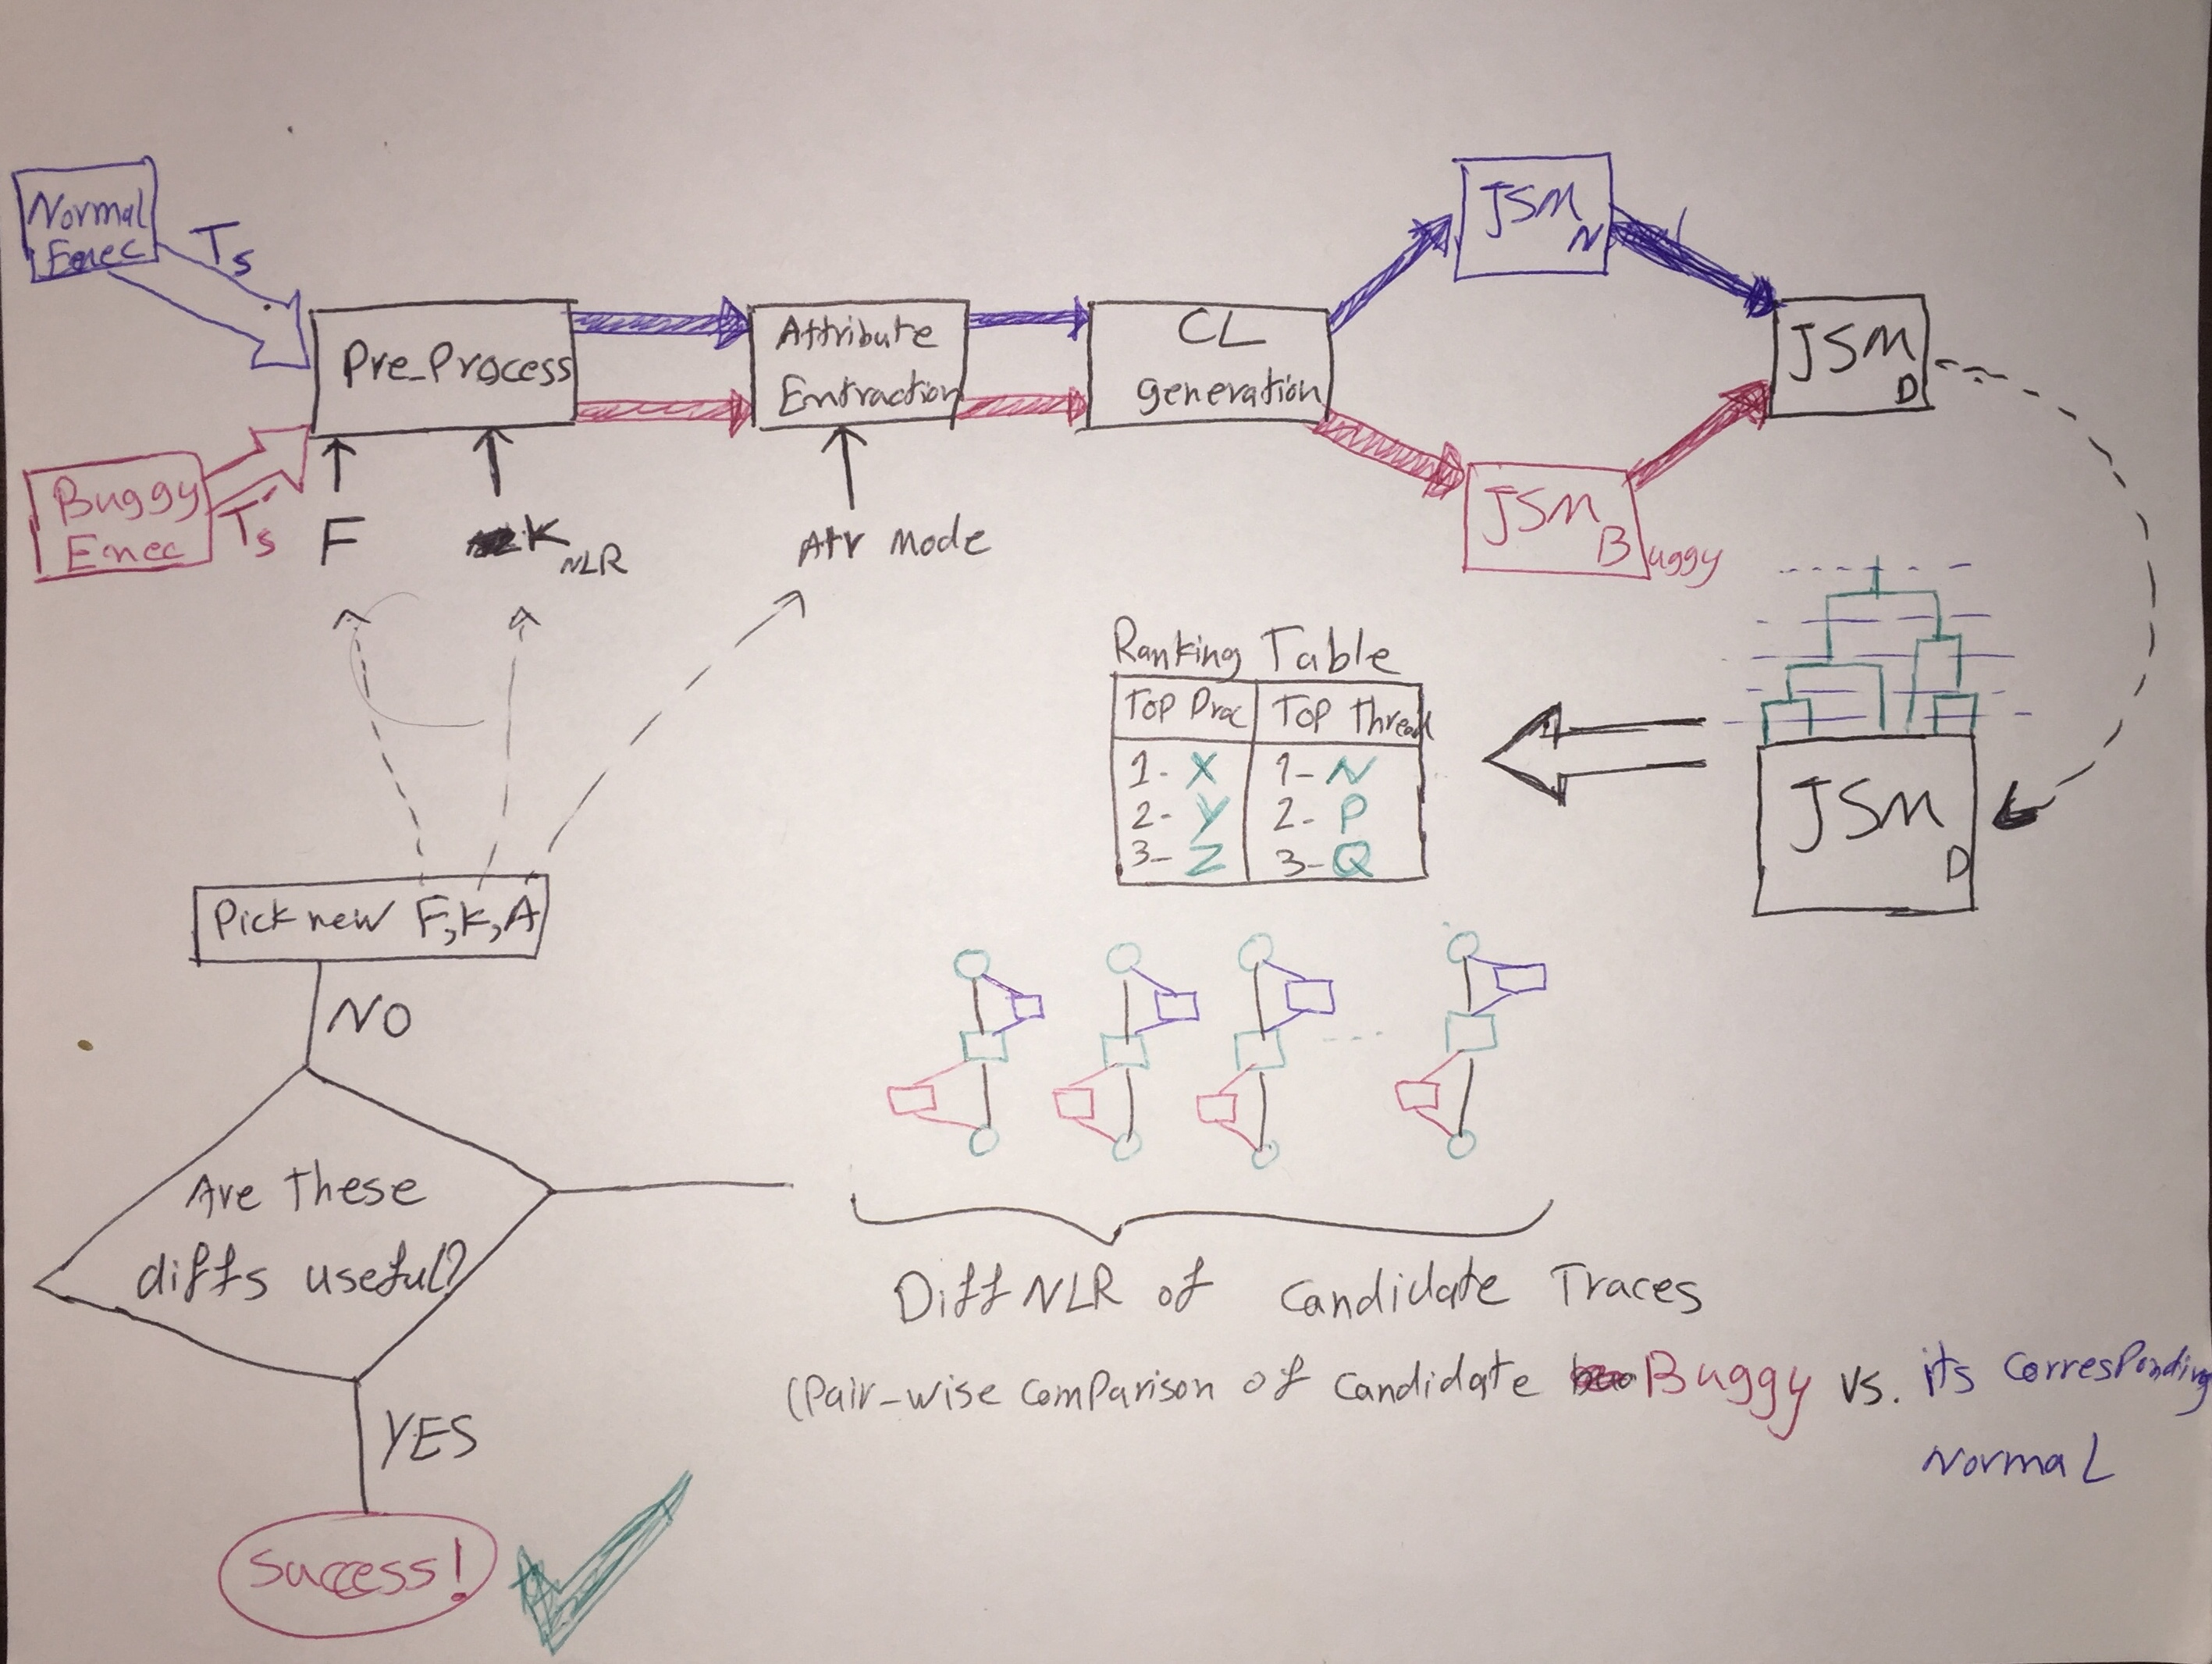
\includegraphics[width=0.95\textwidth]{figs/diffTraceOverview.jpg}
%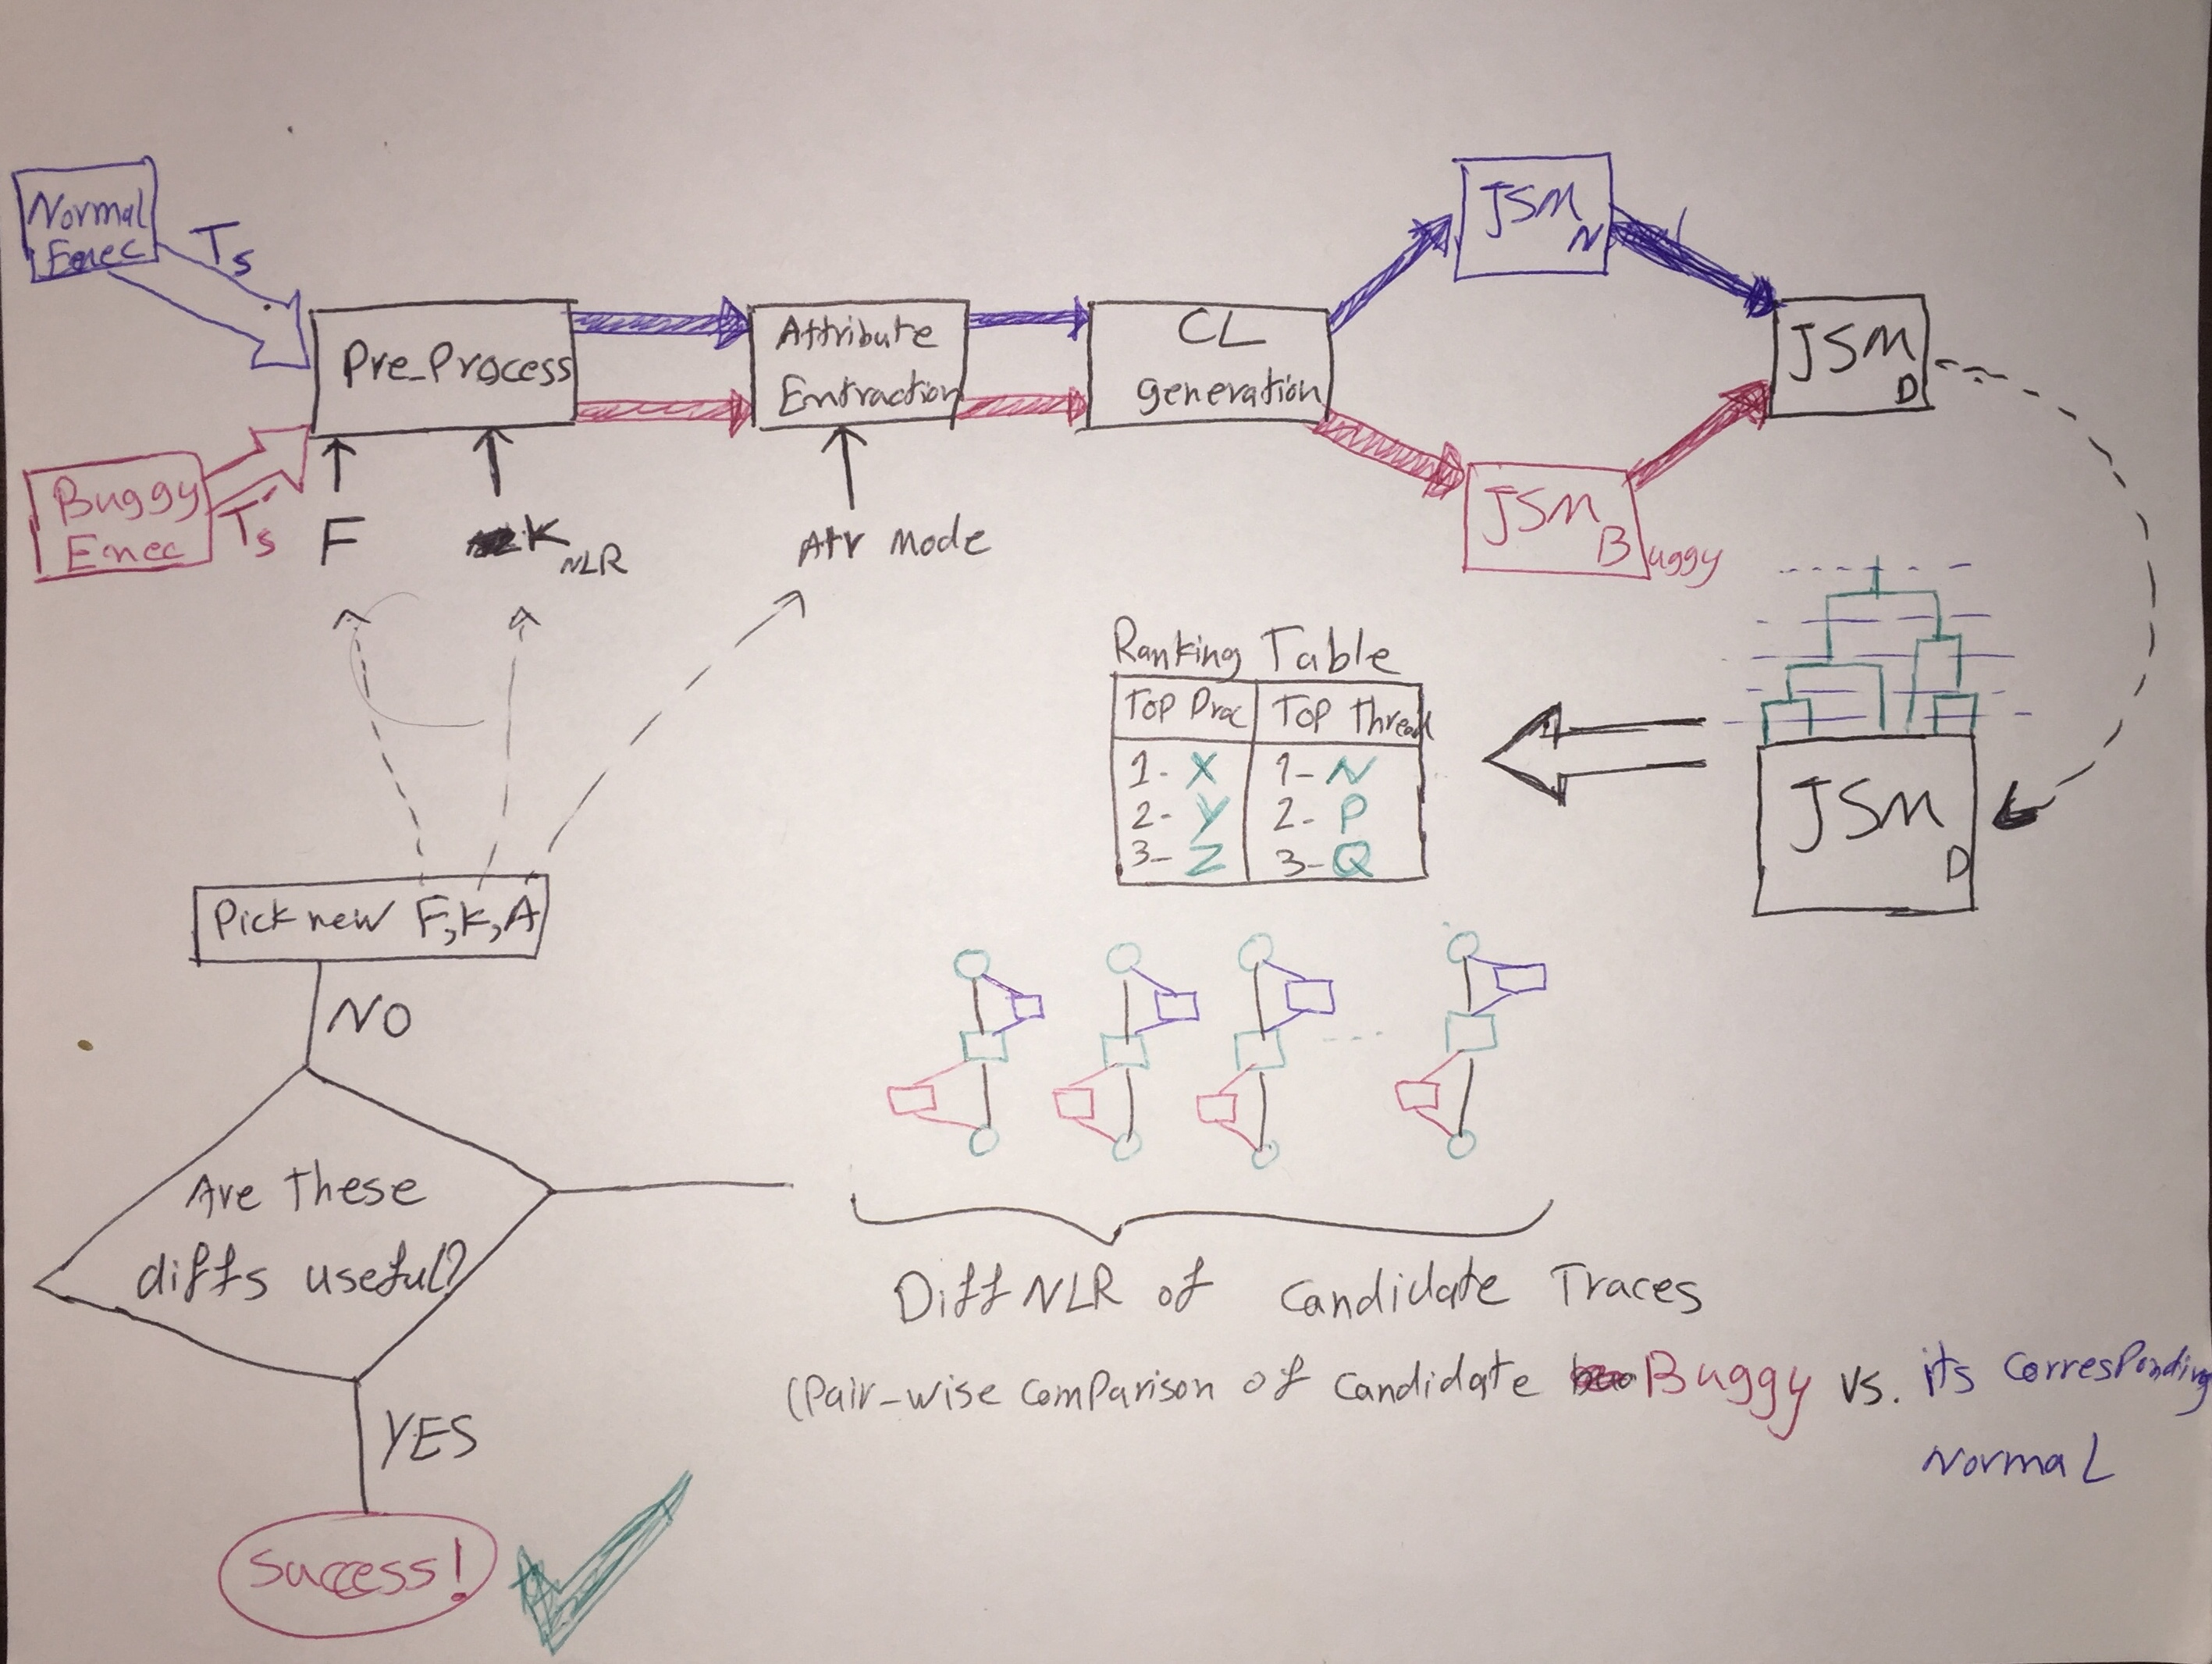
\includegraphics[]{figs/diffTraceOverview.jpg}
\label{fig.diffTraceOverview}
\end{figure*}


\subsection{Trace Pre-processing}
Figure \ref{fig.preprocess} showing the overview of pre-processing chain (decompression, filter, nested loop recognition)


\begin{figure}[]
\caption{Pre-processing Components}
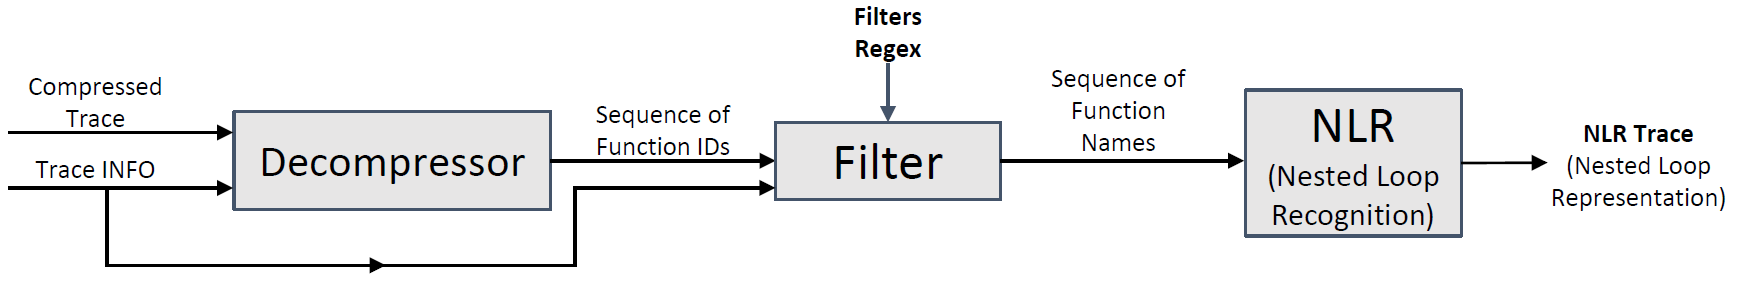
\includegraphics[width=0.49\textwidth]{figs/preprocessChain.png}
\label{fig.preprocess}
\end{figure}


\subsubsection{Decompression and Filter} 
As mentioned earlier, ParLOT incrementally compresses collected sequence of function calls and returns per-thread on-the-fly and store them in form of byte-codes on the disk. Each trace file contains a sequence of function IDs and an INFO file per process holds the corresponding function names.
%
\\
\hl{maybe 1-2 sentences about how decompression works}
\\
Since ParLOT collects the \textit{whole-program} function calls and does not ignore any function, traces might contain functions that we are not interested in studying them at the moment.
%
On the other hand, any piece of information from traces might become handy in later phases of analysis.
%
As an iterative approach, we have a set of pre-defined filters based on the regular expressions and string matching of function calls.
%
On each iteration, we select one or more set of filters and if we get the desired results, we stop. Otherwise, we do our analysis using another, maybe more inclusive, set of filters to see what other information we might gain from traces.
%
Table \ref{tab:filters} shows the built-in filters. One can define custom filters based on the semantics of the application as well.
%
% Please add the following required packages to your document preamble:
% \usepackage{multirow}
\begin{table}[]
\centering
\caption{Applicable filters to PT contents based on regular expressions}
\label{tab:filters}
\scalebox{0.65}{
\begin{tabular}{|c|c|l|}
\hline
\textbf{Category} & \textbf{Sub-Category} & \multicolumn{1}{c|}{\textbf{Description}} \\ \hline
\multirow{2}{*}{Primary} & Returns & Filter out all returns \\ \cline{2-3} 
 & PLT & \begin{tabular}[c]{@{}l@{}}Filter out the ".plt" function calls for external functions/procedures that \\ their address needs to be resolved dynamically from Procedure Linkage \\ Table (PLT)\end{tabular} \\ \hline
\multirow{4}{*}{MPI} & MPI All & Only keep functions that start with "MPI\_" \\ \cline{2-3} 
 & MPI Collectives & Only keep MPI collective calls (MPI\_Barrier, MPI\_Allreduce, etc) \\ \cline{2-3} 
 & MPI Send/Recv & Only keep MPI\_Send, MPI\_Isend, MPI\_Recv, MPI\_Irecv and MPI\_Wait \\ \cline{2-3} 
 & MPI Internal Library & Keep all inner MPI library calls \\ \hline
\multirow{3}{*}{OMP} & OMP All & Only keep OMP calls (starting with GOMP\_) \\ \cline{2-3} 
 & OMP Critical & Only keep OMP\_CRITICAL\_START and OMP\_CRITICAL\_END \\ \cline{2-3} 
 & OMP Mutex & Only keep OMP\_Mutex calls \\ \hline
\multirow{4}{*}{System} & Memory & Keep any memory related functions (memcpy, memchk, alloc, malloc, etc) \\ \cline{2-3} 
 & Network & Keep any network related functions (network, tcp, sched, etc) \\ \cline{2-3} 
 & Poll & Keep any poll related functions (poll, yield, sched, etc) \\ \cline{2-3} 
 & String & Keep any string related functions (strlen, strcpy, etc) \\ \hline
\multirow{2}{*}{Advanced} & Custom & Any regular expression can be captured \\ \cline{2-3} 
 & Everything & Does not filter anything \\ \hline
\end{tabular}}
\end{table}



\subsubsection{Loop Structures} 
\hl{[[WHOLE SUBSECTION NEEDS REWRITE]]}

\begin{itemize}
	\item 1 paragraph: Motivation of detecting loops in traces
	\item 1 paragraph: Loop definition and the original references of NLR algorithm
	\item 1-2 paragraph (or a figure): explaining our variation of NLR algorithm for detecting loop structures in ParLOT traces.
	\item Maybe an illustration on detecting odd/even sort loops
\end{itemize}

HPC applications and resources are of great interest to scientists and engineers for simulating \textit{iterative} kernels. Computer simulation of fluid dynamics, partial differential equations, the Gauss-Seidel method, and finite element methods in form of stencil codes, all include a main outer loop that iterates over some elements (i.e., timesteps) and updates the elements.
%
Loops in source codes would be reflected in traces as sequences of \textit{repetitive patterns}.
%
Mining these repetitive patterns in traces and replacing them with a compact loss-less representation would reveal the structure of sequence of function calls (\hl{or control flow}). 
%
Also a fault in the code might cause a loop to break after some iterations. Thus ``measuring progress'' in each trace, \hl{as it is done as well in PRODOMETER and STAT}, would become handy in later phases. 
%
To recognize loop structures in traces, we have adopted ideas from Kobayashi \cite{kobayashi-84} paper where he defines loops in a sequence of instructions as ``a string of instruction executions in which a particular sequence of distinct instructions (called the \textit{cycle} of the loop) is successively repeated''.
%
This idea have been later expanded by Ketterline et al in \cite{Ketterlin-nlr} where they have introduced Nested Loop Recognition (NLR) algorithm for compressing data access addresses and predicting next accessing addresses.
%
NLR is a memory-bounded algorithm that 

start reading from the beginning of the sequence

store them in the stack

upon each push to stack

	checks for top 3 equal size sub-sequence for isomorphism (equal length and equal corresponding elements)
	
	checks if top n elements of the stack matches with any previous detected loops. if yes, increment the loop count and pop n elements from the stack
	
the above procedure would be repeated any time a change happens in the stack. 

There is a pre-defined size for Max Stack. If stack reaches that point, a fixed number of elements would be popped from the bottom of the stack to free the space for rest of elements.

figure \ref{fig.NLRexample} shows the final product

complexity is $\Theta(K^2N)$ where $K$ is a fixed priori and $N$ is the size of the input. 
%

\begin{figure}[]
\caption{Sample NLR}
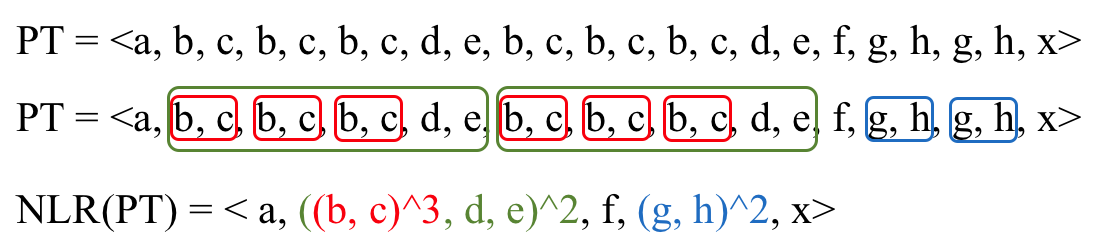
\includegraphics[width=0.45\textwidth]{figs/NLRexample.png}
\label{fig.NLRexample}
\end{figure}



\subsection{Equivalencing Traces via FCA}
\label{subsec:fca}


\begin{itemize}
	\item Construct the context table from example in figure \ref{fig.oddEven}
	\item Construct the Actual Concept Lattice from example in figure \ref{fig.oddEven}
\end{itemize}



\begin{table}[]
\label{tab:sampleContext}
\caption{Context}
\scalebox{0.6}{
\begin{tabular}{l|cccccc}
 & \multicolumn{1}{l}{MPI\_Init()} & \multicolumn{1}{l}{MPI\_Comm\_Size()} & \multicolumn{1}{l}{MPI\_Comm\_Rank()} & \multicolumn{1}{l}{MPI\_Send()} & \multicolumn{1}{l}{MPI\_Recv()} & \multicolumn{1}{l}{MPI\_Finalize()} \\ \hline
Rank 0 & $\times$ & $\times$ & $\times$ &  & $\times$ & $\times$ \\
Rank 1 & $\times$ & $\times$ & $\times$ & $\times$ &  & $\times$ \\
Rank 2 & $\times$ & $\times$ & $\times$ & $\times$ &  & $\times$ \\
Rank 3 & $\times$ & $\times$ & $\times$ & $\times$ &  & $\times$
\end{tabular}}
\end{table}


\begin{figure}[t]
\centering
\scalebox{0.5}{
\includegraphics[width=3.4in]{figs/{sample}.pdf}}
\caption{Sample Concept Lattice from Obj-Atr Context in table\ref{tab:sampleContext}}
\label{fig:sampleCL}
\end{figure}

\begin{figure}[t]
\centering
\scalebox{0.5}{
\includegraphics[width=3.4in]{figs/{sample-reduced}.pdf}}
\caption{Concept Lattice with reduced labels}
\label{fig:sampleCL}
\end{figure}




\begin{itemize}
	\item \hl{1 paragraph background on FCA}
	\item \hl{1-2 paragraphs on advantages of FCA and what we would gain from FCA? Answer: Full pair-wise Jaccard Similarity Matrix (JSM)}
	\item \hl{1 paragraph how JSMs are going to help us (referring to the major figure at the beginning of this section)}
	\begin{itemize}
		\item Some background about Jaccard Similarity Score
		\item How to obtain full pair-wise Jaccard Similarity Matrix (JSM) from a concept lattice (e.g., LCA approach)
	\end{itemize}
	\item \hl{1-2 paragraphs on CL generation (related work and our approach)}
	\begin{itemize}
		\item Batch vs. Incremental \cite{clconst}
		\item Complexity: $O(2^{2K}||E||)$ where $K$ is an upper bound for number of attributes (e.g., distinct function calls in the whole execution) and $||E||$ is the number of objects (e.g., number of PTs).
	\end{itemize}
	\item \hl{1-2 paragraphs (+ 1-2 figures) explaining the FCA ideas on odd/even sort example.}
\end{itemize}



\begin{figure}[]
\centering
\scalebox{0.8}{
\includegraphics[width=3.4in]{figs/{fancy1}.pdf}}
\caption{Pair-wise Jaccard Similarity Matrix (JSM) of MPI processes in Sample code}
\label{fig:jsm}
\end{figure}



Thanks to ParLoT compression mechanism, we are able to efficiently (w.r.t. time and space) collect whole-program function call and return traces (PTs). However, post-mortem analysis of the PTs from thousands of threads requires decompression of traces, and consequently, analysis of large amount of data. Before jumping into \textit{the huge haystack} of PTs to find \textit{the tiny needle} (bug, bug manifestation or root cause of the failure), a middle ground data manipulation is required to simplify and organize the haystack. 

Reducing the search space from thousands of PTs to just a few groups of equivalent PTs (i.e., inter-PT compression) not only requires a similarity measure based on a call matrix but also a scheme that is efficient even for large process counts.
%
Since a pair-wise comparison of all processes is highly inefficient, we use \textit{concept lattices} that stem from \textit{formal concept analysis} (FCA) \cite{clbook} to store and compute groups of similar PTs.
%
FCA can efficiently split the large haystack into a few hay(semi)stacks with ``conceptually'' similar hays in each. This way conceptually isolated PTs (i.e., outliers) which are the potential bug manifestation or root cause would be detected. If no outlier detected, we only have a few distinct group of PTs to dig in, instead of thousands of large traces. With a wider perspective, here are other benefits of FCA for HPC debugging:
\begin{itemize}
\item FCA is scalable and efficient. It can be built incrementally and different kind of information such as full Jaccard Similarity Matrix (JSM) can be generated in linear time due to CL properties.
\item Clustering is only one advantage of creating concept lattices from ParLoT traces. CLs can integrate all traces from an execution to a single entity as signature/model of good or bad execution for further analysis (e.g., prediction) 
\item Due to the \textit{partial order} of nodes within CLs, valuable information can be retrieved from CLs like Happens-Before relation (Vijay Garg’s book explains all applications of FCA in computer science applications)\cite{latticeForDistConst} and machine learning and data mining \cite{Ignatov17})
\end{itemize}

A concept lattice is based on a \textit{formal context} \cite{clbook}, which is a triple $(O, A, I)$, where $O$ is a set of \textbf{objects}, $A$ a set of \textbf{attributes}, and $I \subseteq O \times A$ an incidence relation. The incidence relation associates each object with a set of attributes (e.g., table \ref{tab:sampleContext}).
%
Using FCA for clustering giving us the capability of clustering trace objects based on the ``concept'' of each trace object. We can characterize the ``concept'' (i.e., what we want to understand from the collected traces) by extracting meaningful ``attributes'' from traces. 
%
However, since we are only interested in grouping similar PTs in this work, we only take advantage of similarity measures \cite{Alqadah2011} of concept lattices and leave other properties for future work.
%
Due to typical HPC application topologies such as SPMD, master/worker and odd/even where multiple processes/threads behave similarly, our experiments show that large numbers of PTs can be reduced to just a few groups.
%




\subsection{Suspicious Ranking Table via JSM diffing}

\hl{2-3 paragraphs explaining JSM comparison and how it is going to give us top candidates as suspicious traces to check their gdiff}
\subsection{Parameters}

\hl{2-3 paragraphs explaining the need of iterative approach to go through the tool chain multiple times, each time with different set of parameters (filters, attributes, NLR parameters) to gain insight about different aspects of the application execution (referring to the major overview figure).}